% =========================================================
% TikZ diagram: Open ball vs. Closed ball (side-by-side)
% Place after the Closed Ball definition box.
% Requires: \usepackage{tikz}  \usetikzlibrary{calc}
%           \usepackage{caption}   (for \captionof)
% =========================================================

\begin{center}
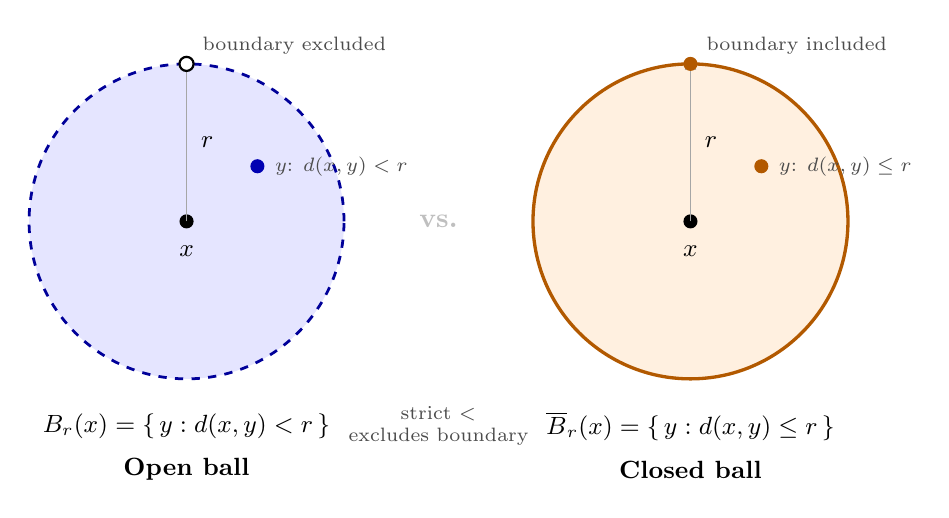
\begin{tikzpicture}[
  dot/.style     = {circle, fill, inner sep=1.8pt},
  opendot/.style = {circle, draw, fill=white, inner sep=1.8pt, line width=0.8pt},
  lbl/.style     = {font=\small},
  sublbl/.style  = {font=\scriptsize, text=gray!60!black}
]

% ---- LEFT PANEL: Open ball ----
\begin{scope}[shift={(-3.2,0)}]
  \fill[blue!10] (0,0) circle (2cm);
  \draw[blue!60!black, dashed, line width=1.0pt] (0,0) circle (2cm);
  \node[dot, fill=black] at (0,0) {};
  \node[lbl, anchor=north] at (0,-0.18) {$x$};
  \draw[->, gray!70, line width=0.6pt] (0,0) -- (0,2);
  \node[lbl, anchor=west] at (0.06, 1.0) {$r$};
  \node[opendot] at (0,2) {};
  \node[sublbl, anchor=south west] at (0.08, 2.0) {boundary excluded};
  \node[dot, fill=blue!70!black] at (0.9, 0.7) {};
  \node[sublbl, anchor=west] at (1.0, 0.7) {$y$: $d(x,y) < r$};
  \node[lbl] at (0, -2.6) {$B_r(x) = \{\,y : d(x,y) < r\,\}$};
  \node[lbl, font=\small\bfseries] at (0, -3.15) {Open ball};
\end{scope}

% ---- VS divider ----
\node[font=\normalsize\bfseries, text=gray!50] at (0, 0) {vs.};
\node[sublbl, align=center] at (0, -2.6)
  {strict $<$\\excludes boundary};

% ---- RIGHT PANEL: Closed ball ----
\begin{scope}[shift={(3.2,0)}]
  \fill[orange!12] (0,0) circle (2cm);
  \draw[orange!70!black, solid, line width=1.2pt] (0,0) circle (2cm);
  \node[dot, fill=black] at (0,0) {};
  \node[lbl, anchor=north] at (0,-0.18) {$x$};
  \draw[->, gray!70, line width=0.6pt] (0,0) -- (0,2);
  \node[lbl, anchor=west] at (0.06, 1.0) {$r$};
  \node[dot, fill=orange!70!black] at (0,2) {};
  \node[sublbl, anchor=south west] at (0.08, 2.0) {boundary included};
  \node[dot, fill=orange!70!black] at (0.9, 0.7) {};
  \node[sublbl, anchor=west] at (1.0, 0.7) {$y$: $d(x,y) \le r$};
  \node[lbl] at (0, -2.6)
    {$\overline{B}_r(x) = \{\,y : d(x,y) \le r\,\}$};
  \node[lbl, font=\small\bfseries] at (0, -3.15) {Closed ball};
\end{scope}

\end{tikzpicture}
\captionof{figure}{Open ball $B_r(x)$ (left) versus closed ball $\overline{B}_r(x)$
(right) in a metric space $(X,d)$.
The dashed boundary of $B_r(x)$ indicates that boundary points satisfying
$d(x,y)=r$ are \emph{excluded} (strict inequality); the solid boundary of
$\overline{B}_r(x)$ indicates they are \emph{included} ($\le$).}
\label{fig:open-closed-balls}
\end{center}